\chapter{Lokalisierungsalgorithmen}
\label{chap:char_localization}
Im Folgenden Kapitel soll die verwendete Algorithmik vorgestellt werden. Dabei wird zunächst ein magnetisch räumliches Signalverarbeitungsmerkmal vorgestellt. Dieses Merkmal wird für eine relative Lokalisierung (Rekonstruktion der einer kinematischen Kette) und eine absolute Lokalisierung innerhalb eines definierten Arbeitsraums genutzt. In diesem Kapitel werden die Sensoren als ideal angenommen, um die algorithmische Herleitung nicht unnötig kompliziert zu machen. 

Es wurde ein iterativer Algorithmus entwickelt, der Vorwissen über die Anatomie integriert und so effizient die Haltung schätzt. Die Prämisse für den Algorithmus ist, dass jedes kinematische Element, mit Ausnahme des ersten, mit einem Magnetfeldsensor ausgestattet wird. Am ersten kinematischen Element ist eine 3D-Spule befestigt. Desweiteren wird zunächst angenommen, dass die Sensorachse diesselbe Orientierung wie das zugehörige kinematische Element und der Sensor genau in der Mitte des kinematischen Elements lokalisiert. Im Allgemeinen hat die Pose eines Sensors fünf Freiheitsgrade, drei für die Position, sowie 2 für die Orientierung der Sensorachse. Durch die Kopplung des Sensors an die Elemente wird die Anzahl der Freiheitsgrade reduziert zur Anzahl der Freiheitsgrade des Gelenks.

Absolute Lokalisierung

\section{Simulationsetup}
Die Herleitung des Algorithmus soll mit kleinen Simulationen veranschaulicht werden. Die Simulation besteht aus drei idealen Dipolquellen, die die verwendete Quelle modellieren, sowie zunächst einem ideal angenommenen Punktsensor. Dies bedeutet, dass der Sensor die Projektion des magnetischen Feldes auf die sensitive Achse des Sensors detektiert. Im späteren Verlauf wird für die Herleitung des Schätzalgorithmus eine kinematische Kette mit bis zu zwei Elementen verwendet. Eine solche Kette ist in Abbildung \ref{fig:Sensorplacement}.

\begin{figure}[h!]
		\centering
		\begin{overpic}[width=\textwidth,trim = 0 0 0 0]{04_lokalisierung/images/Sensorplacement.png}
			\put(0,48){3D-Spule}
			\put(27,27){$\vec{r}\tindex{j1}$}
			\put(59,53){$\vec{r}\tindex{j2}$}
			\put(40,47){$l\tindex{js1}$}
			\put(62,25){$l\tindex{js2}$}
			\put(38,32){Sensor 1}
			\put(59,38){Sensor 2}
		\end{overpic}
		\caption{Sensor- und Quellenanordnung: Die kinematische Kette besteht aus zylinderförmigen Element, sowie Gelenken die diese verbinden und die Möglichkeit haben diese zu bewegen. Die linke Seite zeigt die Anordnung der Quellen und Sensoren auf der kinematischen Kette. Auf dem ersten Element ist eine 3D-Spule angebracht. Die weiteren Elemente sind mit Sensoren ausgerüstet. Diese sind auf der Mittelachse des kinematischen Elements (siehe rechter Teil).
		}
		\label{fig:Sensorplacement}
	\end{figure}

\section{Maximalvektor}
	In der vorgestellten Algorithmik wird ein räumliches Feature eingeführt. Der Hauptgedanke dahinter ist, dass eine kinematische Kette durch die Ausrichtung der einzelnen Elemente beschrieben werden können. Die Ausrichtung der einzelnen Elemente kann in kartesischen Koordinaten mit einem Vektor der Länge 1 beschrieben werden. Die Zielgröße ist dementsprechend eine Anzahl an räumlichen 3D-Vektoren, daher wurde als Eingangsgröße ebenfalls ein räumlicher Vektor ausgewählt.
	Der Maximalvektor (MV) wird wie folgt definiert. Es sei eine dreidimensionale Quelle $\vec{m} = \left[\begin{array}{c} m\tindex{x}\\ m\tindex{y} \\ m\tindex{z}\end{array}\right] $, lokalisiert im Koordinatenursprung, sowie ein Sensor am Ort $\vec{r}$ mit einer Orientierung der sensitiven Achse $\vec{e}_\text{s}$. 
	Ein magnetischer Dipol sei definiert wie folgt [Zitat]
	\begin{equation}
		\vec{B}\tindex{dip}(\vec{r},\vec{m}) = \frac{1}{4\pi r^2}\frac{3\vec{r}(\vec{m}\cdot\vec{r})-\vec{m}r^2}{r^3}.
		\label{eq:magDipolDef}
	\end{equation}
	Ein idealer Sensor misst die Projektion des magnetischen Feldes auf die Sensorachse
	\begin{equation}
		B\tindex{sensor}(\vec{r},\vec{e}_s,\vec{m}) =  \vec{B}\tindex{dip}(\vec{r}) \cdot \vec{e}_s.
		\label{eq:magDipSensor}
	 \end{equation}
	Der MV ist in diesem Fall, die Dipolorientierung $\frac{\vec{m}}{|\vec{m}|}$ für die $B\tindex{sensor}(\vec{r},\vec{e}_s,\vec{m})$ maximal wird.


        
        
\section{Relative Lokalisierung}
In diesem Kapitel wird ein Ansatz aufbauend auf den theoretischen Grundlagen des vorherigen Kapitels vorgestellt. Zunächst wird ein iterativer Ansatz gezeigt, mit dem die Haltung einer kinematischen Kette effizient geschätzt werden kann. Desweiteren werden die Eindeutigkeit, Optimierungen (des Modells und des Rechenbedarfs) und eine Nachverarbeitung vorgestellt. 


\subsection{Iterativer Algorithmus}

    Der Algorithmus kombiniert die magnetischen Zusammenhänge und das Vorwissen über die Anatomie. Die Prämisse des Algorithmus ist, dass bei korrekt angenommener Sensororientierung, mit der Anatomie die korrekte Position des Sensors berechnet werden kann. Mit der korrekten Position kann mithilfe der magnetischen Zusammenhänge die korrekte Sensororientierung bestimmt werden. Diese Selbstkonsistenz wird nun ausgenutzt.

    Für den Algorithmus werden die Position des Gelenks $\vec{r}\tindex{j}$ und die Distanz zwischen Gelenk und Sensor benötigt. Es wird zunächst eine zufällige Orientierung $\vec{\hat{e}}\tindex{s,1}$ des Sensors angenommen. Mit der Anatomie wird die zugehörige Sensorposition bestimmt

    \begin{equation}
        \vec{\hat{r}}\tindex{s,$i$} = \vec{r}\tindex{j} + l\tindex{js} \, \vec{\hat{e}}\tindex{s,$i$} .
        \label{eq:formelIter1}
    \end{equation}
    
    Im nächsten Schritt wird die Sensororientierung für die Position mit den magnetischen Zusammenhängen, die in den Gleichungen \,\ref{eq:formel15} bis \ref{eq:formel18} beschrieben wurden, bestimmt.

    \begin{equation}
        	\vec{\hat{e}}\tindex{s,$i+$1} = \vec{f}(\vec{\hat{r}}\tindex{s,$i$},\vec{e}\tindex{max}).
        \label{eq:formelIter2}
    \end{equation} 
    
    Diese Porzedur wird mit der jeweils neuen Orientierung wiederholt bis die Veränderung der Orientierung einen Schwellwert unterschreitet. Der Ablauf des Algorithmus ist in Abbildung \ref{fig:Flussdiagramm} zu sehen.
    

\begin{figure}[h]
    \centering
    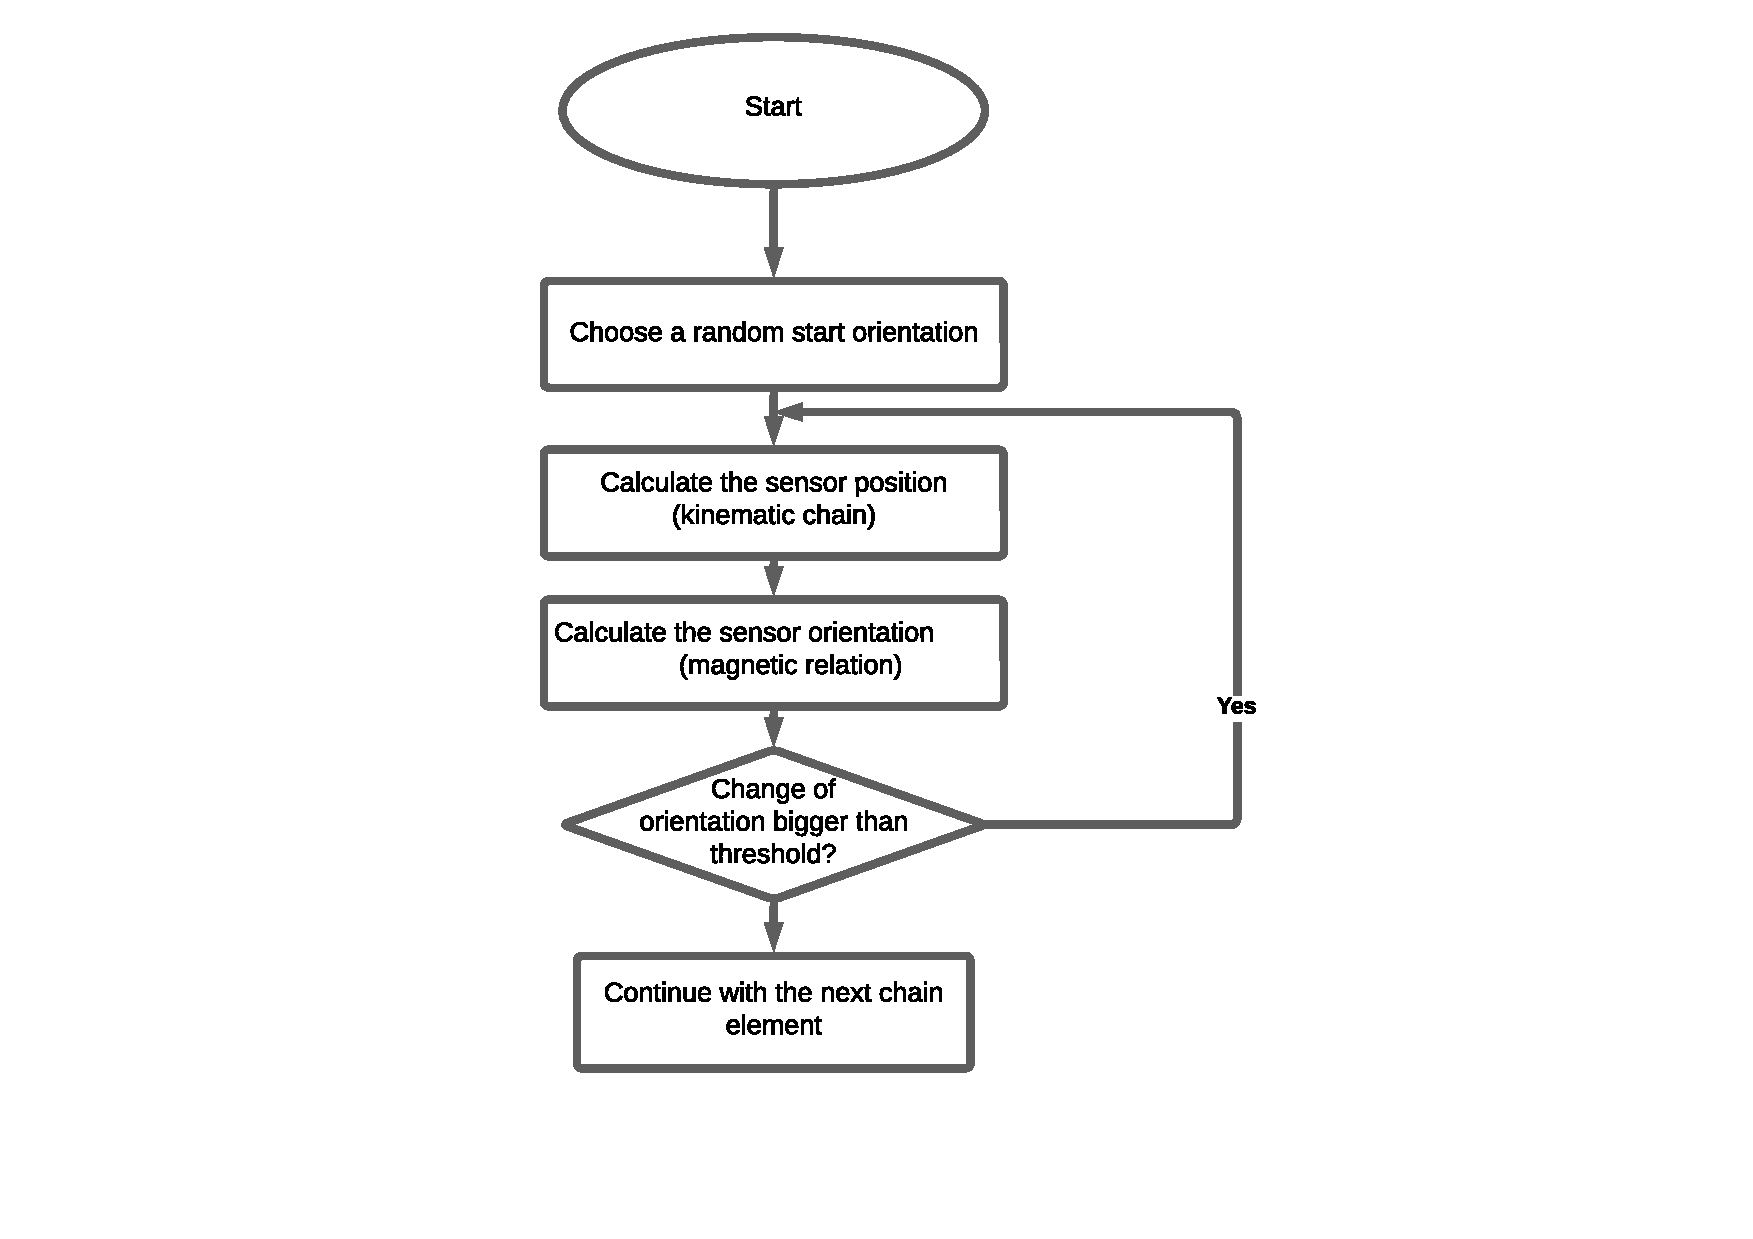
\includegraphics[width=0.5\textwidth,trim = 0 0 0 0]{04_lokalisierung/images/Flussdiagramm.pdf} 
    \caption{Flussdiagramm des iterativen Algorithmus: Der Algorithmus startet mit einer zufällig ausgewählten Sensororientierung. Im ersten Schritt wird die relative Sensorposition bestimmt. Daraus wird die zugehörige Sensororientierung bestimmt. Diese Prozedur wird wiederholt, bis die Veränderung zwischen den Iterationen kleiner ist als ein definierter Schwellenwert und Konvergenz erreicht ist. Diese Orientierung ist dann die geschätzte Lösung.}
    \label{fig:Flussdiagramm}
\end{figure}

	Eine Visualisierung dieser Prozedur ist in Abbildung, wo die Orientierungen und Positionen für die einzelnen Iterationen dargestellt ist. Nach etwa 15 Iterationen stimmt die Sensorpose mit einer potentiellen Pose überein.

\begin{figure}[h]
    \centering
    
    \inputTikZ{0.35}{04_lokalisierung/images/legend.tikz} 
    \label{fig:legend}
    \subfloat[Setup]{
        \begin{overpic}[scale=0.17,trim= 4cm 0 4cm 0]{04_lokalisierung/images/PotentialPoses_for_Inkscape_Setup_grid.png}
            \put(50,45){$x$}
            \put(30,65){$y$}
            \label{fig:Setup}
        \end{overpic}
    }
    \subfloat[Iteration 1]{
        \begin{overpic}[scale=0.17,trim= 4cm 0 4cm 0]{04_lokalisierung/images/PotentialPoses_for_Inkscape_Iteration1_grid.png}
            \label{fig:Iteration1}
        \end{overpic}
    }
    \subfloat[Iteration 2]{
        \begin{overpic}[scale=0.17,trim= 4cm 0 4cm 0]{04_lokalisierung/images/PotentialPoses_for_Inkscape_Iteration2_grid.png}
            \label{fig:Iteration2}
        \end{overpic}
    }
    \subfloat[Iteration 15]{
        \begin{overpic}[scale=0.17,trim= 4cm 0 4cm 0]{04_lokalisierung/images/PotentialPoses_for_Inkscape_Iteration4_grid.png}
            \label{fig:Iteration15}
        \end{overpic}
    }
    \caption{Beispielhafter iterativer Prozess: Diese Abbildung zeigt die Iterationen für einen einfachen Aufbau. Die Unterabbildung \ref{fig:Setup} zeigt den verwendeten Aufbau mit dem Koordinatensystem. Der Ursprung dieses Aufbaus befindet sich am ersten kinematischen Kettenelement, wo sich auch die Quelle befindet. Die Quelle ist mit dem ersten kinematischen Element so verbunden, dass die relative Position der Quelle zur kinematischen Kette immer konstant ist. In den folgenden Abbildungen wurde das Koordinatensystem weggelassen. Die blauen Vektoren stellen die möglichen Posen für die erkannte MV dar. Die hellgrüne Konstruktion zeigt die Bodenwahrheit. Der rote Vektor ist ein normalisierter Positionsvektor des Sensors, der auf die potentielle Pose in dieser Richtung zeigt. Der Sensor ist am zweiten Knochen angebracht. Er wird durch ein schwarzes Rechteck mit einem Vektor in die sensitive Richtung dargestellt. Unterabbildung\,\subref{fig:Iteration1} beginnt mit einer Knochenorientierung in $x$-Richtung. Für einige Iterationen sind die kinematische Kette und der zugehörige Positionsvektor dargestellt. Nach 15 Iterationen (sub-figure\,\subref{fig:Iteration15}) stimmt die Sensorpose mit einer potentiellen Pose (ground truth) überein und der Algorithmus konvergiert.}
    \label{fig:Concept_Algorithm}
\end{figure}

Einfluss der Längenänderungen auf die Konvergenzgeschwindigkeit
Q einfügen

\subsection{Eindeutigkeit der Lösung}
	Im folgenden wird die die Eindeutigkeit des vorgestellten iterativen Algorithmus geprüft. Der Algorithmus ist eindeutig, wenn jedem möglichen Eingangsvektor $\vec{e}\tindex{max}$ eine Sensororientierung $\vec{e}\tindex{s}$ zu geordnet werden kann. Die Eingangs- und Ausgangsvektoren werden dafür in jeweils zwei Winkel aufgeteilt. 

    Der Eingangsvektor besitzt zwei Freiheitsgrade, die die Richtung definieren. Die Orientierung des Sensors wird ebenfalls über zwei Winkel (Freiheitsgrade) definiert. Im folgenden wird zunächst eine Entkopplung der Ein- und Ausgangsvektoren vorgenommen, also hat eine Eingangsgröße nur Einfluss auf eine Ausgangsgröße. Da es sich auf beiden Seiten um Winkel handelt, müssen diesen Winkeln Rotationsachsen zugeordnet werden. 

    Zunächst wird der Zusammenhang aus Kapitel \ref{subsec:Lokalisierungszusammenhänge}, dass $\vec{e}_{max}$, $\vec{e}_s$ und $\vec{e}_r$ in einer Ebene liegen verwendet. Dies bedeutet gleichzeitig auch, dass die Gelenkspostion $\vec{r}_j$ in dieser Ebene liegen muss. Dies ist der Fall, da diese von der Sensorposition in Richtung der Sensororientierung liegt. Daher kann der normalen Vektor $\vec{e}_{n}$ dieser Ebene wie folgt bestimmt werden
    \begin{equation}
        \vec{e}_{n} = \frac{\vec{e}_{max}\times \vec{r}_j}{|\vec{e}_{max}\times \vec{r}_j|}
    \end{equation}

    Dies bedeutet, dass die Sensororientierung auf einer Ebene, einer Ebenschar die durch $\vec{r}_j$ definiert wird. Daher ist die erste Rotationsachse $\frac{\vec{r}_j}{|\vec{r}_j|}$. Die erste Eingangsgröße $\phi_{m,1}$ ist daher der Winkel zwischen $\vec{e}_n$ und einer frei wählbaren Bezugsachse. Die Bezugsachse muss nur senkrecht zu $\vec{r}_j$ stehen. Die Ausgangsgröße $\phi_{s,1}$ entspricht dann der Eingangsgröße.  Dieser Zusammenhang ist in Abbildung \ref{fig:Visualisierung_Uniqueness_Ebene} zu sehen.
    
	\begin{figure}[h!]
		\centering
		\begin{overpic}[width=0.7\textwidth,trim = 0 0 0 0]{04_lokalisierung/images/Visualisierung_Uniqueness_gedreht.pdf}
			\put(82,44){$\phi\tindex{s}$}
			\put(62,25){$\phi$}
			\put(20,14){$\phi\tindex{m}$}
			\put(6,30){$\theta\tindex{m}$}
			\put(13,26){$\vec{m}$}
			\put(90,5){$x$}
			\put(57,60){$y$}
			\put(2,62){$z$}
			\put(40,30){$\vec{r}$}
			\put(75,47){$\vec{e}\tindex{s}$}
		\end{overpic}
		\caption{ Beschreibung des ersten Freiheitsgrades: In der Abbildung ist eine kinematische Kette, bestehend aus zwei Elementen. Im Ursprung ist eine 3D-Spule an der die kinematische Kette angebracht ist. In gelb ist $\vec{e}_{max}$ dargestellt. Dieser spannt gemeinsam mit $\vec{r}_j$ die gelbe Ebene auf. Auf dem zweiten Kettenelement ist ein Sensor in der Mitte des Sensors angebracht und das Gelenk ist so geknickt, dass der Sensor leicht nach unten schaut. Die $XY$-Ebene ist in grau dargestellt. In der Abbildung ist gut zu sehen, dass die gelbe Ebene, durch das erste und zweite ELement schneidet. Es ist erkennbar, dass sowohl $\vec{r}_j$, $\vec{r}_s$ und $\vec{e}_s$ in dieser Ebene liegen.
			}
		\label{fig:Visualisierung_Uniqueness_Ebene}
	\end{figure}
Die Lösung ist nun auf einen Freiheitsgrad eingeschränkt. Der zweite Freiheitsgrad, ist nun der Winkel der um den Normalenvektor dreht. Als Bezugsachse wird im Folgenden ein $\vec{r}_j$ verwendet. Die Eingangsgröße ist dann der Winkel $\phi_{m,2}$ zwischen $\vec{e}_{max}$ und $\vec{r}_j$ und die Ausgangsgröße $\phi_{s,2}$ ist der Winkel zwischen $\vec{e}_s$ und $\vec{r}_j$.
	\begin{figure}[h!]
		\centering
		\begin{overpic}[width=0.7\textwidth,trim = 0 0 0 0]{04_lokalisierung/images/Eindeutigkeit_Ebene.pdf}
			\put(82,44){$\phi\tindex{s}$}
			\put(62,25){$\phi$}
			\put(20,14){$\phi\tindex{m}$}
			\put(6,30){$\theta\tindex{m}$}
			\put(13,26){$\vec{m}$}
			\put(90,5){$x$}
			\put(57,60){$y$}
			\put(2,62){$z$}
			\put(40,30){$\vec{r}$}
			\put(75,47){$\vec{e}\tindex{s}$}
		\end{overpic}
		\caption{
			Winkelzusammenhang: Die Abbildung zeigt den Ebenenschnitt, der gelben Ebene, von Abbildung \ref{fig:Visualisierung_Uniqueness_Ebene}. In der Abbildung ist die kinematische Kette in der von $\vec{e}_{max}$ und $\vec{r}_j$ aufgespannten Ebene. In gelb ist die zweite Eingangsgröße $\phi_{m,2}$ dargestellt. Der blaue Winkel zeigt die Ausgangsgröße $\phi_{s,2}$.
			}
		\label{fig:Visualisierung_Winkelbeschreibung_2}
	\end{figure}

Im Folgenden wird zunächst ein funktionaler Zusammenhang $\phi\tindex{max,2} = f(\phi\tindex{s,2})$ aufgestellt. Zu nächst sei die Gelenksposition $\vec{r}\tindex{j}$ wie folgt definiert, wobei $l\tindex{aj}$, der Distanz von Quelle zu Gelenk entspricht und auf 1 normiert wird um den Zusammenhang später verallgemeinern zu können.  
	\begin{equation}
		\vec{r}\tindex{j} = \left[\begin{array}{c} 1\\ 0 \end{array}\right] 
	\end{equation}
	Die Position des Sensors $\vec{r}\tindex{s}$ kann mit der Länge zwischen Sensor und Gelenk $l\tindex{js}$ wie folgt beschrieben werden.
	\begin{equation}
		\vec{r}\tindex{s} = \left[\begin{array}{c} 1+Q\cos(\phi\tindex{s,2})\\ Q\sin(\phi\tindex{s,2}) \end{array}\right] 
	\end{equation}
	Nun wird zunächst die Winkel zwischen $x$-Achse und $\vec{r}\tindex{s}$ bestimmt.
	\begin{equation}
		\phi\tindex{r} = \arctan\big(\frac{Q\cos(\phi\tindex{s,2})}{1+Q\sin(\phi\tindex{s,2})}\big)
	\end{equation}
	mit Gleichung \ref{eq:relMaxS} kann nun $\phi\tindex{max,2}$ bestimmt werden 
	\begin{equation}
		\phi\tindex{max,2} = -\arctan(\frac{1}{2} \tan(\phi\tindex{s,2} - \phi\tindex{r} ).
        \label{eq:uniqness_Value_2}
	\end{equation}
	
	
\begin{figure}
	\begin{subfigure}{0.5\textwidth}
	\scalefont{4}
		\centering
		\inputTikZ{0.225}{04_lokalisierung/images/q0_05_Unique.tikz}
		\caption{$0<Q<=0.5$}
		\label{fig:0_05_Unique}
	\end{subfigure}
	\hspace{0.25cm}
	\begin{subfigure}{0.5\textwidth}
	\scalefont{4}
		\centering
		\inputTikZ{0.225}{04_lokalisierung/images/q05_10_Unique.tikz}
		\caption{$0.5<Q<=1$}
		\label{fig:05_10_unique}
	\end{subfigure}
	\begin{subfigure}{0.5\textwidth}
	\scalefont{4}
		\centering
		\inputTikZ{0.225}{04_lokalisierung/images/q11_16_Unique.tikz}
		\caption{$1<Q$}
		\label{fig:bigger1_unique}
	\end{subfigure}
	\caption{ Funktionaler Winkelzusammenhang: In der Abbildung ist der Zusammenhang zwischen $\phi\tindex{s,2}$ und $\phi\tindex{max,2}$ für verschiedene Wertebereiche von $Q$. Die Abbildungen \ref{fig:0_05_Unique} und \ref{fig:bigger1_unique} zeigen eine eindeutige Zuordnung zwischen $\phi\tindex{s,2}$ und $\phi\tindex{max,2}$. In diesem Bereich gibt es für jeden Eingangsvektor einen zugehörigen Ausgangsvektor. In Abbildung \ref{fig:05_10_unique} ist der Zusammenhang für $0.5 < Q < 1$ zu sehen. Hier ist teilweise einem Wert für $\phi\tindex{max,2}$ zwei unterschiedliche Werte für $\phi\tindex{s,2}$ zugeordnet.}

    
	\label{fig:uniqueness}
\end{figure}

Dieser Zusammenhang ist nicht trivial und nicht einfach umkehrbar. In einem Skript wurde mit einer Auflösung von $1°$ Verläufe für Gleichung \ref{eq:uniqness_Value_2} für unterschiedliche $Q$ bestimmt. Die Ergebnisse sind in Abbildung \ref{fig:uniqueness} dargestellt. Aus der Abbildung geht hervor, dass der Algorithmus eindeutige Ergebnisse für $Q<=0.5$ und $Q>1$ liefert. In der späteren Anwendung muss dies beachtet werden, wobei bei einer SensorGlove Anwendung die kinematischen Elemente relativ klein ist. Dies führt zu einem kleinen $l\tindex{js}$ und somit zu einem kleinerem $Q$. 

\subsection{Analyse der benötigten Rechenleistung}
Analyse mit einer Matlabsimulation

\subsection{Optimierungen}
    Laufzeitoptimierung(LookUpTable), Korrektur von Modellfehlern (Dicke des Fingers, Verdrehung des Sensors)
    Diskussion...
	\subsection{Analyse der Unsicherheiten}
		Einführung virtuelle/mechanische Achsen,        

	\section{Absolute Lokalisierung}
		\subsection{Grundsätzliche Gedanken}
		\subsection{Ebenenschnitt}
		\subsection{Orientierung}
		

	
